% Standalone XeLaTeX source. Uses standard commands and distributed packages.
% Source problem: public/notes/物工/問題/2016ap_exam.pdf, PDF pages 11–12.
\documentclass[11pt,a4paper]{article}
\usepackage[margin=24mm]{geometry}
\usepackage{fontspec}
\usepackage{xeCJK}
\setCJKmainfont{HaranoAjiMincho-Regular.otf}
\setCJKsansfont{HaranoAjiGothic-Medium.otf}
\usepackage{amsmath,amssymb}
\usepackage{tikz}
\usetikzlibrary{arrows.meta}
\setlength{\parindent}{1em}
\setlength{\parskip}{0.35em}
\renewcommand{\figurename}{図}
\title{物理工学専攻 院試解答集 ver2\\2016年 物理学II 第4問}
\author{政岡凜太郎}
\date{}
\begin{document}
\maketitle

\section*{[1] 電子線の加速電圧}
相対論的補正を無視すると電子の運動量は$p=\sqrt{2meV}$であり、ド・ブロイ関係$p=h/\lambda$より
\begin{equation}
 V=\frac{h^2}{2me\lambda^2}.
\end{equation}
$\lambda=0.01\,\mathrm{nm}=1.0\times10^{-11}\,\mathrm m$を代入すると
\begin{equation}
 V=\frac{(6.6\times10^{-34}\,\mathrm{J\,s})^2}
 {2(9.1\times10^{-31}\,\mathrm{kg})(1.6\times10^{-19}\,\mathrm C)(1.0\times10^{-11}\,\mathrm m)^2}
 =1.5\times10^4\,\mathrm V.
\end{equation}

\section*{[2] 有限正方格子の散乱振幅}
左下の格子点を原点に取ると、原子位置は$\boldsymbol r_{n_x,n_y}=(a n_x,a n_y,0)$である。従って振幅は二つの有限和に分離する。
\begin{align}
 A(\boldsymbol K,N_x,N_y)
 &=f\sum_{n_x=0}^{N_x-1}e^{-iaK_xn_x}
    \sum_{n_y=0}^{N_y-1}e^{-iaK_yn_y}\\
 &=fL(K_x,N_x)L(K_y,N_y),\\
 L(K,N)&=\sum_{n=0}^{N-1}e^{-iaKn}
 =e^{-iaK(N-1)/2}\frac{\sin(NaK/2)}{\sin(aK/2)}.
\end{align}
分母がゼロとなる点では極限を取る。したがって
\begin{equation}
 |L(K,N)|^2=\left[\frac{\sin(NaK/2)}{\sin(aK/2)}\right]^2,
\end{equation}
また$N=1,2,3$ではそれぞれ$1$、$4\cos^2(aK/2)$、$[1+2\cos(aK)]^2$となる。
\begin{figure}[htbp]
\centering
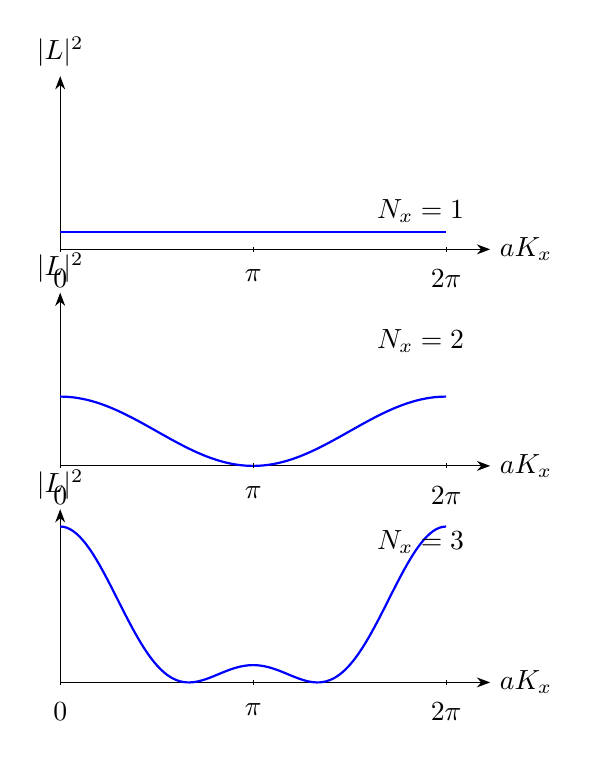
\begin{tikzpicture}[xscale=0.78,yscale=0.22,>=Stealth]
 \begin{scope}
   \draw[->] (0,0)--(7.0,0) node[right] {$aK_x$};
   \draw[->] (0,0)--(0,10) node[above] {$|L|^2$};
   \draw[thick,blue,domain=0:6.283,samples=120] plot (\x,1);
   \node[anchor=west] at (5.0,2.2) {$N_x=1$};
   \draw (0,0.15)--(0,-0.15) node[below=3pt] {$0$};
   \draw (3.142,0.15)--(3.142,-0.15) node[below=3pt] {$\pi$};
   \draw (6.283,0.15)--(6.283,-0.15) node[below=3pt] {$2\pi$};
 \end{scope}
 \begin{scope}[yshift=-12.5cm]
   \draw[->] (0,0)--(7.0,0) node[right] {$aK_x$};
   \draw[->] (0,0)--(0,10) node[above] {$|L|^2$};
   \draw[thick,blue,domain=0:6.283,samples=120] plot (\x,{4*cos(\x r/2)^2});
   \node[anchor=west] at (5.0,7.2) {$N_x=2$};
   \draw (0,0.15)--(0,-0.15) node[below=3pt] {$0$};
   \draw (3.142,0.15)--(3.142,-0.15) node[below=3pt] {$\pi$};
   \draw (6.283,0.15)--(6.283,-0.15) node[below=3pt] {$2\pi$};
 \end{scope}
 \begin{scope}[yshift=-25cm]
   \draw[->] (0,0)--(7.0,0) node[right] {$aK_x$};
   \draw[->] (0,0)--(0,10) node[above] {$|L|^2$};
   \draw[thick,blue,domain=0:6.283,samples=120] plot (\x,{(1+2*cos(\x r))^2});
   \node[anchor=west] at (5.0,8.1) {$N_x=3$};
   \draw (0,0.15)--(0,-0.15) node[below=3pt] {$0$};
   \draw (3.142,0.15)--(3.142,-0.15) node[below=3pt] {$\pi$};
   \draw (6.283,0.15)--(6.283,-0.15) node[below=3pt] {$2\pi$};
 \end{scope}
\end{tikzpicture}
\caption{$|L(K_x,N_x)|^2$の一周期。各パネルの縦軸は実際の強度である。}
\end{figure}

\section*{[3] 単原子三角格子の回折}
図3の基本格子ベクトルは
\begin{equation}
 \boldsymbol a_1=a\begin{pmatrix}\sqrt3/2\\1/2\end{pmatrix},\qquad
 \boldsymbol a_2=a\begin{pmatrix}-\sqrt3/2\\1/2\end{pmatrix}.
\end{equation}
逆格子は$\boldsymbol a_i\cdot\boldsymbol b_j=2\pi\delta_{ij}$で定めるから
\begin{equation}
 \boxed{\boldsymbol b_1=\frac{2\pi}{a}\begin{pmatrix}1/\sqrt3\\1\end{pmatrix},\qquad
 \boldsymbol b_2=\frac{2\pi}{a}\begin{pmatrix}-1/\sqrt3\\1\end{pmatrix}}.
\end{equation}
面内の原子位置$\boldsymbol r=n_1\boldsymbol a_1+n_2\boldsymbol a_2$を散乱振幅の位相因子$e^{-i\boldsymbol K\cdot\boldsymbol r}$に代入すると、二方向の有限等比和が得られる。多数の単位胞で双方の和が強め合う条件は$\boldsymbol K_{\parallel}\cdot\boldsymbol a_i=2\pi m_i$（$m_i$は整数）である。したがって散乱ベクトルの面内成分は逆格子ベクトル$\boldsymbol G=m_1\boldsymbol b_1+m_2\boldsymbol b_2$であり、
\begin{equation}
 |\boldsymbol G|^2=\frac{16\pi^2}{3a^2}
 (m_1^2+m_2^2+m_1m_2).
\end{equation}
括弧内は$(m_1-m_2)^2+3m_1m_2$とも書けるので、3で割った余りは$0$か$1$であり、値$2$は取らない。指数$(1,0)$、$(1,1)$、$(2,0)$でそれぞれ$1,3,4$となるため、最小の三つの正の値は$1,3,4$である。垂直入射では$\boldsymbol k$は面に垂直で、$\boldsymbol G$は$\boldsymbol k'$の面内成分なので、回折角$\theta$（入射・散乱波数ベクトル間の全角）には
\begin{equation}
 |\boldsymbol G|=|\boldsymbol k'|\sin\theta=k\sin\theta,\qquad k=\frac{2\pi}{\lambda}
\end{equation}
が成り立つ。三殻がいずれも前方の検出面に届く条件は、最大の$|\boldsymbol G|$に対して$4\lambda/(\sqrt3a)<1$、すなわち$0<\lambda/a<\sqrt3/4$である。この範囲で、小さい方から三つの角は
\begin{equation}
 \boxed{\theta_1=\sin^{-1}\!\left(\frac{2\lambda}{\sqrt3a}\right),\qquad
 \theta_2=\sin^{-1}\!\left(\frac{2\lambda}{a}\right),\qquad
 \theta_3=\sin^{-1}\!\left(\frac{4\lambda}{\sqrt3a}\right)}.
\end{equation}
散乱が可能な範囲で各回折角は$0<\theta<\pi/2$である。小角度では$\theta_1\simeq2\lambda/(\sqrt3a)$、$\theta_2\simeq2\lambda/a$、$\theta_3\simeq4\lambda/(\sqrt3a)$となる。

各逆格子殻には六つの等価なベクトルがあるため、平面ディテクタ上では入射方向を中心とする三つの六回対称なスポット列となる。小角近似では検出面上の半径が$\theta_j$に比例し、その比は$1:\sqrt3:2$である。第1殻と第3殻は$x$軸から$60^\circ$おきに並び、第2殻はそれらから$30^\circ$回転している。
\begin{figure}[htbp]
\centering
\begin{tikzpicture}[scale=0.56]
 % Detector coordinates are the reciprocal vectors, normalized by the
 % first-shell radius.  The integer-index condition selects each full shell.
 \pgfmathsetmacro{\shellscale}{sqrt(3)/2}
 \begin{scope}[xshift=-5.0cm]
   \draw[->] (-3.4,0)--(3.3,0) node[right] {$x$};
   \draw[->] (0,-3.1)--(0,3.2) node[above] {$y$};
   \fill (0,0) circle (2.4pt);
   \foreach \m in {-2,-1,0,1,2} {\foreach \n in {-2,-1,0,1,2} {
     \pgfmathtruncatemacro{\q}{\m*\m+\n*\n+\m*\n}
     \ifnum\q=1\relax
       \pgfmathsetmacro{\gx}{\shellscale*(\m-\n)/sqrt(3)}
       \pgfmathsetmacro{\gy}{\shellscale*(\m+\n)}
       \fill (\gx,\gy) circle (2.4pt);
     \fi
     \ifnum\q=3\relax
       \pgfmathsetmacro{\gx}{\shellscale*(\m-\n)/sqrt(3)}
       \pgfmathsetmacro{\gy}{\shellscale*(\m+\n)}
       \fill (\gx,\gy) circle (2.4pt);
     \fi
     \ifnum\q=4\relax
       \pgfmathsetmacro{\gx}{\shellscale*(\m-\n)/sqrt(3)}
       \pgfmathsetmacro{\gy}{\shellscale*(\m+\n)}
       \fill (\gx,\gy) circle (2.4pt);
     \fi
   }}
   \node at (0,-3.7) {(a) 位置（$\theta_1,\theta_2,\theta_3$）};
 \end{scope}
 \begin{scope}[xshift=5.0cm]
   \draw[->] (-3.4,0)--(3.3,0) node[right] {$x$};
   \draw[->] (0,-3.1)--(0,3.2) node[above] {$y$};
   \fill (0,0) circle ({sqrt(3)*2.4pt});
   \foreach \m in {-2,-1,0,1,2} {\foreach \n in {-2,-1,0,1,2} {
     \pgfmathtruncatemacro{\q}{\m*\m+\n*\n+\m*\n}
     \pgfmathsetmacro{\gx}{\shellscale*(\m-\n)/sqrt(3)}
     \pgfmathsetmacro{\gy}{\shellscale*(\m+\n)}
     \ifnum\q=1\relax
       \fill (\gx,\gy) circle (2.4pt);
     \fi
     \ifnum\q=3\relax
       \fill (\gx,\gy) circle ({sqrt(3)*2.4pt});
     \fi
     \ifnum\q=4\relax
       \fill (\gx,\gy) circle (2.4pt);
     \fi
   }}
   \node at (0,-3.7) {(b) 基底強度（面積比 $1:3:1$）};
 \end{scope}
\end{tikzpicture}
\caption{小角近似での三殻の回折位置。(b)は[4]で求めるハニカム基底の相対強度を点の面積で表す。}
\end{figure}

\section*{[4] ハニカム構造の基底干渉}
図4の二原子基底の相対位置を$\boldsymbol\tau=(2\boldsymbol a_1+\boldsymbol a_2)/3$とする。$f_A=f$、$f_B=2f$と選べば、逆格子点$\boldsymbol G=m_1\boldsymbol b_1+m_2\boldsymbol b_2$での基底振幅は
\begin{equation}
 F_{\rm basis}=f_A+f_Be^{-i\boldsymbol G\cdot\boldsymbol\tau}
 =f\left[1+2e^{-i(2\pi/3)(2m_1+m_2)}\right].
\end{equation}
従って単位胞数による共通因子を除くと
\begin{equation}
 I_{\rm basis}=|F_{\rm basis}|^2/|f|^2
 =5+4\cos\!\left(\frac{2\pi}{3}(2m_1+m_2)\right).
\end{equation}
各殻のすべての指数について$t=2m_1+m_2$と置くと、$t^2\equiv m_1^2+m_2^2+m_1m_2\pmod 3$である。したがって第一・第三殻では$t\not\equiv0\pmod3$、第二殻では$t\equiv0\pmod3$となる。上の余弦は順に$-1/2,1,-1/2$であり、各殻のどのピークも強度$3,9,3$をもつ。その比は
\begin{equation}
 \boxed{I_1:I_2:I_3=1:3:1}.
\end{equation}
第二殻のピークは他の二殻より3倍強い。

\section*{[5] 面直積層による干渉}
隣接層の間隔を$d$、積層数を$N_z$とする。全ての層で同じ面内原子配置を持ち、散乱ベクトルの垂直成分を$c=K_z$とすれば、各層の位相差は$cd$である。振幅には
\begin{equation}
 S_{N_z}(c)=\sum_{j=0}^{N_z-1}e^{-icjd}
 =e^{-icd(N_z-1)/2}\frac{\sin(N_zcd/2)}{\sin(cd/2)}
\end{equation}
が掛かる。$cd=2\pi m$（$m$整数）では各層が同位相となり、$|S_{N_z}|^2=N_z^2$である。この条件の近くの最初の零点は$cd=2\pi m\pm2\pi/N_z$なので、ピーク幅は$c$について$1/(N_zd)$の程度になる。一方、層条件からの位相のずれを固定すると
\begin{equation}
 \frac{|S_{N_z}(c)|^2}{N_z^2}
 \leq \frac{1}{N_z^2\sin^2(cd/2)}.
\end{equation}
従って$N_z|\sin(cd/2)|\gg1$なら、強め合うピークに比べて強度が小さい。有限層では、層条件から外れた振幅が一般に厳密にゼロになるわけではない。

垂直入射では$\boldsymbol k=(0,0,k)$であり、面内回折ベクトルを$\boldsymbol G$とすると、弾性散乱の前方解は
\begin{equation}
 \boldsymbol k'=(\boldsymbol G,\sqrt{k^2-|\boldsymbol G|^2}),\qquad
 c=k'_z-k=\sqrt{k^2-|\boldsymbol G|^2}-k.
\end{equation}
非零の$\boldsymbol G$に対するこの$c$が層条件のピーク幅以上に外れると、層からの散乱は弱め合い、回折ピークが抑えられる。垂直入射でも層条件に近い場合には抑制されないが、問題文の消失は層条件から外れた場合に対応する。

傾斜によって層条件と弾性散乱を両立できる具体例として、$0<|\boldsymbol G|<2k$のとき、入射の面内成分を$-\boldsymbol G/2$に取ると
\begin{equation}
 \boldsymbol k=\left(-\frac{\boldsymbol G}{2},\sqrt{k^2-\frac{|\boldsymbol G|^2}{4}}\right),\qquad
 \boldsymbol k'=\left(\frac{\boldsymbol G}{2},\sqrt{k^2-\frac{|\boldsymbol G|^2}{4}}\right).
\end{equation}
両波数の大きさは$k$で、$\boldsymbol k'-\boldsymbol k=(\boldsymbol G,0)$となる。従って$c=0$、すなわち$m=0$の層条件が満たされ、全層が強め合う。面直方向からの入射の傾斜角は
\begin{equation}
 \alpha=\sin^{-1}\!\left(\frac{|\boldsymbol G|}{2k}\right)
 \simeq\frac{|\boldsymbol G|}{2k}\qquad (|\boldsymbol G|/k\ll1)
\end{equation}
であるため、小角回折の領域では小さな傾斜でピークが現れる。これは選んだ$\boldsymbol G$に対応する方位と角度の構成である。
\end{document}
